\documentclass[11pt]{article}

\usepackage[utf8]{inputenc}
\usepackage[T1]{fontenc}
\usepackage[margin=1in]{geometry}
\usepackage{amsmath}
\usepackage{amssymb}
\usepackage{graphicx}
\usepackage{subcaption}
\usepackage{booktabs}
\usepackage{placeins}

\usepackage[blocks]{authblk}

\usepackage{hyperref}

\graphicspath{{image/}}

\title{FaceKit: a Lightweight Toolkit for Interpretable Facial Phenotyping in Rare Diseases}

\renewcommand\Authfont{\normalsize}
\renewcommand\Affilfont{\small}
\setlength{\affilsep}{0.4em}

\author[1,2]{Hongzhuo Chen}
\author[1,2]{Zhanliang Wang}
\author[3,4]{Florent Pollet}
\author[3,4,5]{Gamze Gürsoy}
\author[1,6,*]{Kai Wang}

\affil[1]{Raymond G. Perelman Center for Cellular and Molecular Therapeutics,
Children's Hospital of Philadelphia, Philadelphia, USA}

\affil[2]{Applied Mathematics and Computational Science Graduate Program,
University of Pennsylvania, Philadelphia, USA}

\affil[3]{Department of Biomedical Informatics, Columbia University,
NYC, USA}

\affil[4]{New York Genome Center, NYC, USA}

\affil[5]{Department of Computer Science, Columbia University,
NYC, USA}

\affil[6]{Department of Pathology and Laboratory Medicine,
Perelman School of Medicine, University of Pennsylvania,
Philadelphia, PA 19104, USA}

\affil[*]{Corresponding author:
\href{mailto:wangk@chop.edu}{\texttt{wangk@chop.edu}}}

\date{}

\begin{document}

\maketitle

\begin{abstract}
% Superseded first version of the abstract, kept here for reference:
% Facial phenotypes are important indicators in the characterization of many rare genetic diseases. Although the Human Phenotype Ontology provides standardized terminology for describing facial phenotypic features, many of these features lack standardized and reproducible methods for quantitative measurement from facial images. FaceKit is a lightweight interpretable toolkit that converts facial images into structured, quantitative representations of facial morphology. It integrates facial landmark extraction, pose quality filtering, geometric normalization, landmark visualization, cohort average-face generation, and 120 facial measurements, while supporting disease-aware feature selection and user-defined feature extensions.
Facial phenotyping plays an important role in the diagnosis and clinical characterization of rare genetic diseases, many of which are associated with recognizable craniofacial features. However, traditional approaches for describing facial morphology rely largely on qualitative clinical observation and free-text descriptions, which are often subjective, non-standardized, and difficult to reproduce across observers and institutions. Although the Human Phenotype Ontology (HPO) provides controlled terms for describing dysmorphic facial features, these terms are typically categorical rather than quantitative and may vary depending on examiner experience and interpretation. Here, we present FaceKit, a computational framework for quantitative facial phenotyping from frontal facial photographs. FaceKit extracts standardized measurements of facial landmarks and derived 120 morphological features, then reports feature-level z-scores representing deviation from population reference distributions. To support ancestry-aware phenotyping, we constructed reference models using the FairFace dataset as a control population spanning diverse ancestry groups. We further evaluated FaceKit using multiple rare disease facial phenotype resources, including GMDB, RDFace, and an internal clinical cohort. In addition to quantitative facial analysis, FaceKit includes synthetic facial image generation to support rare disease model development and data augmentation. We also performed privacy evaluation to assess whether synthetic images reveal identifiable information from real patient photographs and could therefore compromise patient privacy. Across disease case studies, FaceKit-derived quantitative measurements captured known facial features associated with rare genetic disorders and provided objective support for clinical phenotype interpretation. We further demonstrate that FaceKit can assist human reviewers in generating HPO terms and text-based descriptions of facial features from patient photographs, improving consistency and reproducibility of facial phenotype annotation. Together, these results establish FaceKit as a useful tool for rare disease research, quantitative dysmorphology, and AI-assisted phenotyping. By converting facial morphology into standardized, quantitative, and interpretable features, FaceKit has the potential to improve rare disease diagnosis, support genotype-phenotype studies, and enable more reproducible clinical characterization across diverse patient populations.
\end{abstract}

\noindent\textbf{Keywords:} facial phenotyping, rare disease, facial photo, landmarking, privacy evaluation

\section{Introduction}
Facial morphology is an important component of phenotypic characterization in many rare genetic diseases and can provide useful signals for disease recognition alongside other clinical and genetic information. Traditionally, these patterns have been assessed through expert observation and described using standardized phenotype terminology such as the Human Phenotype Ontology (HPO). More recently, neural-network \cite{DeepGestalt,hsieh2022gestaltmatcher} and vision-language models \cite{mint, gestaltmml} have also used facial images to support rare-disease recognition and the identification of facial phenotype terms.

However, existing approaches do not fully address the need for quantitative and interpretable facial phenotyping. HPO terms provide a standardized vocabulary, but many facial features are still evaluated qualitatively and are not directly linked to reproducible measurements from images. Similarly, learning-based models commonly produce disease rankings, probabilities, or phenotype labels, while the facial characteristics underlying these outputs are often difficult to express. General-purpose facial landmark tools provide image coordinates, but researchers must still define their own normalization procedures, geometric measurements, feature-selection rules, and output formats. This fragmentation makes it difficult to compare facial morphology consistently across patients, diseases, and study cohorts.

To address this gap, we developed FaceKit, a lightweight and interpretable toolkit that converts facial images into structured quantitative representations of facial morphology. FaceKit integrates facial landmark extraction and visualization, frontal-pose quality filtering, geometric normalization, and cohort average-face generation. It computes 120 interpretable measurements across major facial regions and supports disease-aware feature selection for downstream cohort analysis. FaceKit also provides an extensible framework through which researchers can define additional geometric features while maintaining a unified output representation. Together, these functions provide a reproducible pipeline for transforming facial images into quantitative phenotypic features for rare-disease research.

\section{Methods}

FaceKit provides an integrated workflow for processing, quantitatively characterizing, and augmenting rare-disease facial image datasets. The workflow begins with image preprocessing and landmark-based facial phenotyping. In addition to producing interpretable geometric measurements for individual- and cohort-level analysis, this stage generates standardized facial images, landmark representations, and structured features that can be used as inputs for downstream machine-learning and generative-model development. Building on these standardized images, FaceKit supports the training and application of cohort-specific generative models to produce synthetic facial images for data augmentation and methodological development. The generated images can subsequently be processed through the same phenotyping workflow to evaluate whether they preserve the geometric characteristics of the corresponding disease cohorts. Finally, because the pre-trained generators are intended for distribution and reuse, FaceKit includes a privacy-assessment framework that evaluates whether synthetic images reproduce identifiable information or exhibit excessive similarity to the real patient photographs used for training.


\subsection{Image Preprocessing}

FaceKit accepts facial images provided either in a single directory or in a hierarchical directory structure organized by disease cohort. Each image is first processed using MediaPipe Face Landmarker to detect 478 two-dimensional facial landmarks and estimate a facial transformation matrix. The transformation matrix is converted into yaw, pitch, and roll angles to assess whether the image is sufficiently frontal for subsequent geometric analysis. By default, images with an absolute yaw or pitch greater than $15^{\circ}$, or an absolute roll greater than $10^{\circ}$, are marked as non-frontal. This quality-control procedure reduces variation introduced by head pose and identifies images for which facial measurements may be unreliable. For each image, FaceKit stores the landmark coordinates together with the image identifier and dimensions. The extracted data can be saved as individual JSON files or combined into a JSONL file for batch processing and downstream phenotype extraction.

\subsection{Landmark visualization}

FaceKit provides visualization functions for inspecting facial landmark extraction results on individual images. Detected landmarks can be rendered as a connected facial mesh or as landmark-only points overlaid on the original image. Users can optionally display specific landmark groups, including facial contours and iris landmarks, to examine particular facial regions in greater detail. These visualizations support manual inspection of landmark placement, identification of potential detection failures, and verification of image suitability before downstream geometric phenotype extraction.

\subsection{Geometric Phenotype Extraction}

FaceKit converts the extracted facial landmarks into structured quantitative
representations of facial morphology. Before feature calculation, landmark
coordinates are geometrically normalized to reduce variation caused by image
position, orientation, and scale.

Head pose is removed first. Under an orthographic camera, the image abscissa of a
landmark at head-frame position $(X, Y, Z)$ viewed at angle $\theta$ is
$x_{\mathrm{img}} = X\cos\theta + Z\sin\theta$
(Fig.~\ref{fig:posecorr-arms}\subref{fig:posecorr-geom}). The first term is an
anisotropic scaling of the face plane and cancels in any ratio of two
measurements taken in that plane; the second term does not, and it is the only
one that requires a depth. Recovering $(X, Y)$ therefore amounts to inverting

\begin{equation}
\begin{pmatrix} X \\ Y \end{pmatrix}
  = \bigl(R_{[:2,\,:2]}\bigr)^{-1}
    \left[ \begin{pmatrix} x \\ y \end{pmatrix} - R_{[:2,\,2]}\, Z \right],
\label{eq:derot}
\end{equation}

where $R$ is the head rotation. FaceKit obtains $R$ from the $3\times3$ block of
the MediaPipe facial transformation matrix, replaced by its nearest pure
rotation through singular-value decomposition; this discards the scale and shear
that make the raw block unsafe to invert as a rotation.

Equation~\eqref{eq:derot} still requires a depth $Z$ for every landmark, and this
is the one quantity a single photograph does not supply. FaceKit takes it from a
fixed canonical-face table of 478 constants, the same table for every image,
rather than from the per-image $z$ that the landmark detector returns
(Fig.~\ref{fig:posecorr-mech}). That per-image estimate is a by-product of
fitting a supervised mesh, not a depth measurement: across the 4,559 images used
here it correlates with the mean-face depth profile at a median $r=0.95$ and only
17.8\% of its energy is image-specific. Reading it back therefore injects
photograph-specific variance into the features, and doing so measurably reduces
the intra-patient reliability of the resulting measurements below the level
obtained with no pose correction at all (Section~\ref{sec:posecorr}). The
canonical table was constructed as the mean de-rotated depth over the same
cohort, so it uses only the component of the detector's depth output that is
stable across images. Setting $Z = 0$ instead, which corresponds to treating the
face as flat and using the pose angles alone, leaves the residual
$Z\sin\theta$ term untouched and is shown below to be worth nothing.

When no transformation matrix is available, the correction degrades to a
roll-only alignment from the eye landmarks; which of the two paths was taken is
recorded for every image, so runs are never pooled across the two conventions.
The pose-corrected configuration is then translated to a common reference
position at the midpoint of the inner canthi. Scale normalization is performed
using anatomically defined reference measurements, including bizygomatic width,
facial height, midface height, and mouth width, depending on the facial region
and feature being measured.

Using the normalized landmarks, FaceKit calculates 120 interpretable geometric features describing regional and global facial morphology. These features include distances, ratios, angles, thickness measurements, curvature--related measurements, asymmetry indices, and facial proportions across the eyebrows, eyes, nose, philtrum, mouth and lips, chin and jaw, forehead, midface and cheeks, and the overall face. Each feature is defined using explicit landmark combinations and geometric operations, allowing its value to be directly inspected and compared across individuals or cohorts.

For disease--organized datasets, FaceKit supports disease-aware feature selection to retain measurements considered relevant to the corresponding disease while preserving a consistent output structure across samples. User-provided disease names can be normalized to MONDO identifiers, with resolved mappings cached for reuse and candidate terms suggested when an exact match is unavailable. Features not selected for a given disease are represented as missing values rather than removed from the output table. FaceKit also allows users to specify additional landmark-based measurements through an input argument or a JSON configuration file, enabling custom features to be incorporated into the same structured feature representation.

\subsection{Average-face generation}

FaceKit generates average-face representations to summarize shared facial morphology within an image cohort. Facial images are first aligned to a common landmark configuration to reduce variation in position, orientation, and scale, after which the aligned images are combined into a cohort-level average. Users can specify the output resolution and optionally apply edge smoothing, a transparent background, or blending with a destination face. The resulting average face provides an intuitive visual summary of common facial patterns within a cohort and can facilitate qualitative comparisons across disease groups.

\subsection{Synthetic Facial Image Generation}

FaceKit additionally supports the generation of synthetic facial images.
Two usage modes are provided. Users with a sufficiently large image
collection can train a generator on their own cohort and sample from the
resulting weights, while other users can sample
directly from generators pre-trained on ten rare-disease cohorts and
distributed with FaceKit.

Facial photographs collected for rare-disease research are often
retrospective and heterogeneous in acquisition quality, and the images used
for training are therefore standardized beforehand. Images that cannot be
used for morphological modelling may optionally be excluded at this stage,
including those obscured by privacy blocks, those of extremely low quality,
and those in which facial features are not clearly visible. Grayscale or
colour-degraded photographs are then colorized using DDColor~\cite{ddcolor},
and blurred or low-resolution faces are restored and upsampled using
GFPGAN~\cite{gfpgan}. Finally, FaceKit locates the facial region from the
detected landmarks, removes the surrounding background, and resizes the
retained facial area to $256\times256$ pixels, so that all training images
share a common facial framing and resolution. This preparation applies to
the training corpus only and is not required when sampling from an existing
generator.

Generators are trained using StyleGAN3~\cite{stylegan3}. A latent vector
$z \sim \mathcal{N}(0, I)$ is transformed by a mapping network into an
intermediate style vector, which modulates the convolutions of a synthesis
network to produce an image, while a discriminator is trained in parallel to
distinguish real from generated images; the two networks are optimized
adversarially (Fig.~\ref{fig:syngen}). Each cohort, comprising on average more than one hundred
prepared images, is trained separately at $256\times256$ resolution with an
R1 regularization weight of $\gamma = 2$, horizontal-flip augmentation
enabled to increase effective data diversity, and a training length of
5{,}000 kimg. The generator and discriminator learning rates are initialized
at $2.5\times10^{-3}$ and $2\times10^{-3}$, respectively, and follow a
cosine decay schedule. Synthetic images are then obtained by drawing latent
vectors from the standard normal distribution and passing them through
either a user-trained or a pre-trained generator.

\begin{figure}[t]
  \centering
  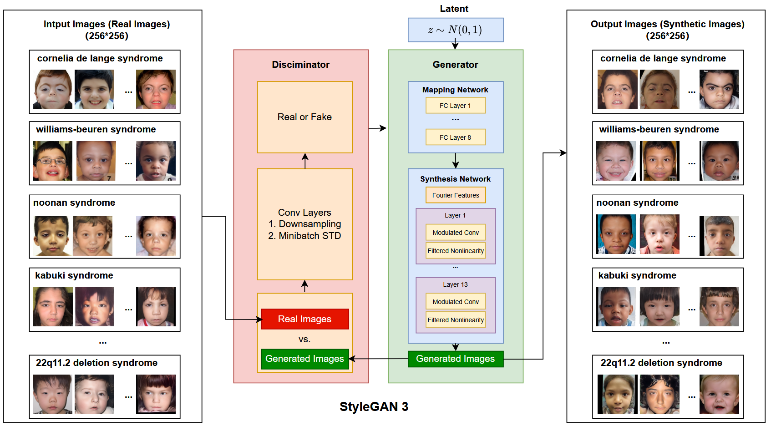
\includegraphics[width=\linewidth]{image/synthetic_image_generation.png}
  \caption{\textbf{Synthetic facial image generation.} Prepared real images of
  each rare-disease cohort (left) are used to train a StyleGAN3 generator. The
  discriminator applies successive downsampling convolutions with a minibatch
  standard-deviation layer and separates real from generated images, while the
  generator maps a latent vector $z \sim \mathcal{N}(0, I)$ through an
  eight-layer mapping network into a style vector that modulates the
  convolutions of the synthesis network. Sampling from the trained generator
  yields $256\times256$ synthetic facial images for the corresponding cohort
  (right).}
  \label{fig:syngen}
\end{figure}

\subsection{Privacy assessment of the pre-trained generators}

Because the generators distributed with FaceKit are trained on photographs of
real individuals, the synthetic images they produce are assessed before release
for residual similarity to the training data. Two aspects are examined
separately: whether a synthetic image reproduces the identity of a training
individual, and whether it reproduces the appearance of a training photograph.

For the identity assessment, the prepared images of each cohort are divided into
a training partition, which is used to fit the generator, and a held-out
partition, which is disjoint from it at the patient level and never enters
generator training. Synthetic images are then sampled from the corresponding
generator. Faces are detected with InsightFace~\cite{insightface}, and the five
detected keypoints are used to align each face to a $112\times112$ crop through
a similarity transform. Identity embeddings are extracted with
ArcFace~\cite{arcface}, and the entire procedure is repeated with
AdaFace~\cite{adaface}, using an IR-50 backbone trained on MS1MV2, and with
LVFace~\cite{lvface}, using the LVFace-L model trained on Glint360K, so that the
assessment does not depend on a single recognition model; images in which no
face is detected are excluded. Distances between embeddings are measured as
cosine distances, and every synthetic and every held-out image is characterized
by its distance to the nearest training image of the same cohort. Rather than
fixing a verification threshold in advance, the threshold is read off the
held-out distribution: for a given percentile $p$, it is set to the $p$-th
percentile of the held-out nearest-neighbour distances, so that the operating
point corresponds to a fixed false-acceptance rate among real images of that
cohort. The proportion of synthetic images falling below this threshold is
recorded at $p = 1$, $2$, $5$, $10$ and $20$. The ordinal behaviour of each
embedding model is verified on the same images: same-person pairs are formed
from images of one patient acquired no more than half a year apart, and each
such pair is compared against a sample of different-person pairs drawn from the
same cohort, checking whether the same-person distance is the smaller one
throughout.

The appearance assessment follows the same design with a perceptual rather than
an identity metric. LPIPS distances~\cite{lpips} are computed with an AlexNet
backbone on images resized to $256\times256$, and each synthetic and held-out
image is compared exhaustively against every training image of its cohort,
retaining the smallest distance; thresholds are again taken from the percentiles
of the held-out distribution. Both assessments are finally summarized by the
nearest neighbour adversarial accuracy~\cite{nnaa}. For two sets of images, the
adversarial accuracy is the proportion of images whose nearest neighbour in the
other set is farther away than their nearest neighbour within their own set,
averaged over the two directions, so that a value of one half indicates that the
two sets cannot be distinguished by proximity. It is evaluated between the
synthetic images and the training partition, and between the synthetic images
and the held-out partition, and the difference between the two, termed the
privacy loss, expresses whether synthetic images lie closer to the training data
than held-out real images of the same cohorts do. The quantity is computed with
embedding distances and with LPIPS distances, pooled across cohorts, and
confidence intervals are obtained by resampling images with replacement.
% TODO: state the bootstrap replicate count once the face_audit run log is available
% (the shipped config default of 10 is a smoke-test value).

\section{Results}

We evaluated FaceKit along the three major components of its workflow. First, we assessed whether the landmark-derived geometric measurements captured facial phenotypes represented by clinically annotated HPO terms and whether these measurements supported interpretable comparisons across patients and disease cohorts. Second, we examined whether the cohort-specific generative models preserved the geometric phenotype distributions of the real images used for training, both within individual disease cohorts and in the differences that distinguish one cohort from another. Finally, because the pre-trained generators are intended for distribution and reuse, we evaluated whether their synthetic outputs reproduced the identities or visual appearance of the real patient photographs used during training. Together, these analyses assess the phenotypic validity, generative fidelity, and privacy characteristics of the FaceKit workflow.

\subsection{Quantitative measurements reproduce annotated facial phenotypes}

We applied FaceKit to a curated subset of the GestaltMatcher Database comprising
4,559 frontal facial images from 50 rare-disease cohorts. For each image, FaceKit
extracted 478 facial landmarks and computed 120 unitless geometric measurements.
After pose filtering and collapsing each patient to the median of their frontal
images, 2,897 patients remained. To express every measurement on a common,
clinically interpretable scale, we built a normative reference from 2,051 FairFace
control images spanning three ancestry groups, of which 886 passed the same pose
filter, and converted each measurement into a $z$-score relative to that reference.
Each of the 97 facial HPO terms in the FaceKit vocabulary is mapped to one
measurement together with the direction in which that measurement is expected to
change, so a signed $z$-score can be read directly as agreement or disagreement
with the annotation.

Of the 97 terms, 84 were carried by at least one patient with a gold-standard
annotation; the remaining 13 had no annotated patient anywhere in the cohort and
could not be assessed. Across the 84 assessable terms, the mapped measurement
deviated from the healthy reference in the direction predicted by HPO for 62
(73.8\%; binomial $p=1.5\times10^{-5}$), with a mean absolute deviation of 0.47
reference standard deviations. The remaining 16 terms showed no clear directional deviation and were considered inconclusive, whereas six deviated in the opposite direction. Among the terms with a clear directional signal, FaceKit agreed with the HPO-predicted direction for 62 of 68 terms (91.2%).

% Restricting attention to the 78 terms carried by
% enough patients to admit a statistical test, 33 reached significance after
% Benjamini--Hochberg correction, 39 did not separate from the reference, and 6
% deviated significantly in the direction opposite to the one HPO predicts. Agreement
% was not driven by the terms with the most annotation: terms carried by 10--29
% patients agreed as often as those carried by 30 or more (82.4\% versus 79.5\%).

To illustrate how the quantitative facial phenotyping module operates, we used hypertelorism in Crouzon syndrome as a case study. Hypertelorism is represented in FaceKit by the inter-pupillary distance normalized by bizygomatic width, calculated as the ratio of the distance between the two iris centres to the distance between the two zygomatic points (Fig.~\ref{fig:ipd}\subref{fig:ipd-crouzon},\subref{fig:ipd-costello}). This example demonstrates how facial landmarks are converted into an interpretable geometric measurement that can be evaluated at both the individual-patient and disease-cohort levels. Across the 238 patients annotated with the term,
this ratio was elevated by 1.04 reference standard deviations
($q=4.2\times10^{-22}$), and among all 120 measurements it was the most
deviant in these same patients, indicating that the signal is specific to the
measurement the term is mapped to rather than a general distortion of the face.
The same ordering is visible at the cohort level: mean normalized inter-pupillary
distance was 0.532 in the Crouzon syndrome cohort against 0.465 across the
remaining cohorts, the highest of the 50 diseases (Fig.~\ref{fig:ipd}\subref{fig:ipd-bars}). Panels \subref{fig:ipd-crouzon} and \subref{fig:ipd-costello} contrast a Crouzon patient with a patient from a cohort at the centre of the same
distribution, with the two landmark pairs entering the ratio drawn on the image.

\begin{figure}[t]
  \centering
  \begin{subfigure}[b]{0.27\linewidth}
    \centering
    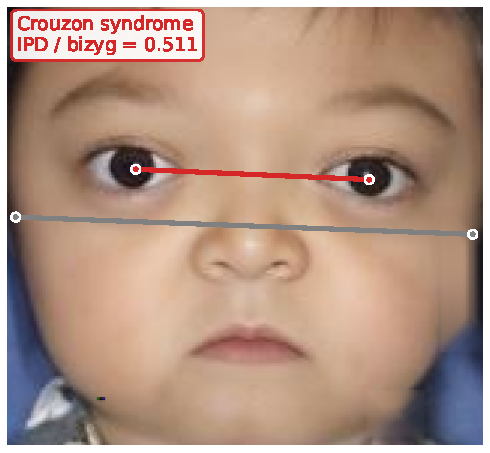
\includegraphics[width=\linewidth]{image/F1a_face_crouzon}
    \caption{}
    \label{fig:ipd-crouzon}
  \end{subfigure}
  \hfill
  \begin{subfigure}[b]{0.27\linewidth}
    \centering
    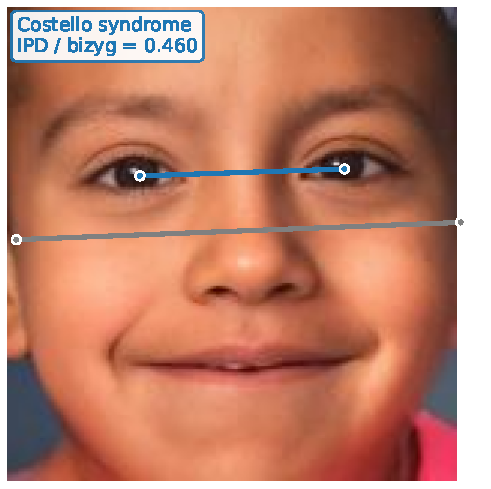
\includegraphics[width=\linewidth]{image/F1b_face_costello}
    \caption{}
    \label{fig:ipd-costello}
  \end{subfigure}
  \hfill
  \begin{subfigure}[b]{0.4\linewidth}
    \centering
    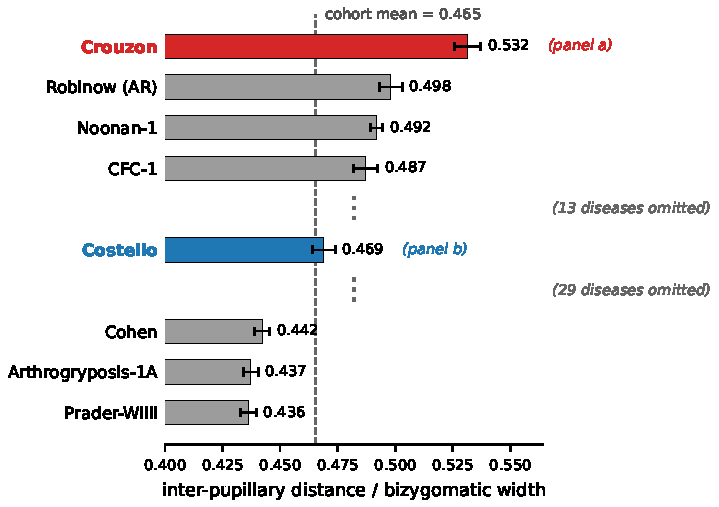
\includegraphics[width=\linewidth]{image/F1c_ipd_bars}
    \caption{}
    \label{fig:ipd-bars}
  \end{subfigure}

  \caption{\textbf{A single FaceKit measurement, from image to cohort.}
  (\subref{fig:ipd-crouzon}, \subref{fig:ipd-costello}) The inter-pupillary
  distance normalized by bizygomatic width, drawn on the images it is computed
  from: the coloured line joins the two iris centres (landmarks 468 and 473) and
  the grey line joins the two zygomatic points (landmarks 234 and 454); the
  measurement is the ratio of their lengths. (\subref{fig:ipd-crouzon}) A patient
  with Crouzon syndrome, the cohort with the highest mean value.
  (\subref{fig:ipd-costello}) A patient with Costello syndrome, a cohort at the
  centre of the same distribution, shown for contrast.
  (\subref{fig:ipd-bars}) Mean normalized inter-pupillary distance per disease
  cohort. Bars give the cohort mean with its standard error; the dashed line marks
  the mean over the remaining cohorts. Of the 50 cohorts, the four highest, the
  three lowest and Costello syndrome are shown, and the rest are omitted as
  indicated. Values are computed on images passing the frontal-pose filter.}
  \label{fig:ipd}
\end{figure}

The six measurements that moved against their annotation share a single
explanation, and it is not that the annotations are wrong. Deviations in this
paragraph are reported as raw measurement $z$-scores, positive meaning a larger
measurement, rather than oriented to the direction the term predicts. In each
case the annotated patients were barely distinguishable from the patient cohort
as a whole:
patients annotated with a narrow nasal bridge measured $+0.82$ against a
cohort-wide baseline of $+0.53$, facial asymmetry $-0.63$ against $-0.48$, and full
cheeks $-0.65$ against $-0.56$. For the other three the annotated patients were in
fact closer to the reference than the average patient: synophrys $+0.41$ against
$+0.52$, a narrow forehead $+0.37$ against $+0.56$, and ptosis $+0.16$ against
$+0.35$. These are therefore not phenotype effects with an inverted sign but
cohort-wide offsets in the measurement itself, which happen to point away from the
direction the term predicts.

Each offset has an identifiable source. Every asymmetry measurement, not only the
one mapped to facial asymmetry, was systematically lower in patients than in
controls (13 of 14 such columns negative, mean $-0.27$). This is a property of the
reference rather than of the patients: an asymmetry measurement is driven by
whatever head pose survives the frontal gate (mean $r=+0.45$ against $|$yaw$|$
across the 15 asymmetry columns), and the FairFace controls carry more residual
pose than the patient photographs do after the same gate (mean $|$yaw$|$
$6.1^{\circ}$ against $4.1^{\circ}$). Stratified by $|$yaw$|$ the two populations
almost coincide (0--3$^{\circ}$: 0.032 against 0.037; 3--6$^{\circ}$: 0.050
against 0.055; 6--9$^{\circ}$: 0.074 against 0.081), so the apparent deficit is
the reference being measured under looser acquisition conditions, not a face that
is genuinely more symmetric. Cheek area is normalized by the square of bizygomatic width, and the
patients annotated with full cheeks did have broader and rounder faces
(face aspect ratio $+0.34$, roundness $+0.29$ against cohort baselines of $+0.07$
and $+0.11$); the denominator therefore grows with the phenotype and inverts the
ratio, the same failure mode that normalization by a phenotype-sensitive scale
produces elsewhere. For synophrys, the measurement is the gap between the medial
brow endpoints, but synophrys is hair occupying that gap, and the landmark mesh
carries no photometric information: the brow points are placed by the shape prior
rather than by the hair boundary. Consistent with this, the brows of these patients
did differ from the reference in shape, but in a different measurement
(medial flare $-0.75$) than the one the term is mapped to. The two weakest cases
are weak for reasons that are visible in the result itself: for ptosis the mapped
measurement ranks 88th of the 120 in these patients, so it is not among the
measurements that deviate at all and reaches significance only through the number
of patients carrying the term ($n=138$), while a narrow forehead is significant
only marginally ($q=0.047$) and is measured from landmarks that lie under the
hairline, where the mesh has no image evidence to place them and where residual
pose dependence remains high ($|r|=0.46$ against pitch, 12th of the 120
measurements). Only the
narrow nasal bridge result rests on few patients ($n=19$), and it uses landmark
indices that have not been verified against the canonical face model.

These six cases indicate that a measurement should be interpreted against the
patient population as well as against healthy controls, since a cohort-wide offset
can produce a confident result in either direction, and that normalization scales
must be chosen so that the denominator is not itself altered by the phenotype being
measured.

\subsection{Depth for pose correction is better taken from a canonical face than
from the image}
\label{sec:posecorr}

The normalization in Equation~\eqref{eq:derot} needs a depth for every landmark,
and a single photograph does not supply one. We compared four ways of answering
that question, differing only in the depth they assume and sharing all 120
feature formulas, so that any difference between them is attributable to the
depth term alone. Arm~A applies no pose correction beyond a roll alignment from
the eye landmarks. Arm~B sets $Z = 0$, treating the face as flat and using the
pose angles alone. Arm~C uses the canonical-face table. Arm~D uses the per-image
$z$ returned by the landmark detector, scaled by a factor previously tuned
against intra-patient reliability.

Arms B and C are the same estimator evaluated at $Z = 0$ and at
$Z = Z^{\mathrm{canon}}$, which removes any difference of implementation from
the comparison. On synthetic faces, where the true depth is known exactly and the
reconstruction can be scored directly, the canonical table recovers the frontal
configuration essentially without error, while the flat-face assumption does not
improve on leaving the pose uncorrected: at a pitch of $25^{\circ}$ the residual
landmark error is 4.82\% of bizygomatic width uncorrected, 5.06\% under the
flat-face assumption and 0.00\% with the canonical table, and under a combined
pitch and yaw of $20^{\circ}$ the three are 6.12\%, 5.81\% and 0.35\%
(Fig.~\ref{fig:posecorr-arms}\subref{fig:posecorr-roundtrip}). This is the
expected consequence of the decomposition above rather than a surprise: with
$Z = 0$ the correction reduces to an anisotropic scaling of the face plane, and
every FaceKit measurement is a ratio in which such a scaling largely cancels.

On the 4,559 real images the four arms were scored on the subset of measurements
for which independent validity evidence exists, so that the comparison is not
diluted by measurements never shown to measure anything. Two of the three
endpoints require no annotation at all: the absolute correlation between a
measurement and the head-pose angle, which a correct normalization should reduce,
and the intra-patient intraclass correlation across repeat photographs of the
same patient, which sets a ceiling on any downstream model. The third is the area
under the curve for separating patients annotated with a term from those who are
not, on the term-measurement pairs that survived both validity contrasts
(Table~\ref{tab:posearms}).

\begin{table}[t]
  \centering
  \caption{\textbf{Four pose-correction arms on 4,559 GMDB images.}
  Correlations with pitch and yaw and the intraclass correlation (ICC) are means
  over the 13 measurements with independent validity evidence; AUC is the mean
  over the six term--measurement pairs that passed both validity contrasts.
  Lower is better for the pose correlations, higher for ICC and AUC.}
  \label{tab:posearms}
  \begin{tabular}{llccc c}
    \toprule
    Arm & Depth $Z$ & $|r|$ pitch & $|r|$ yaw & ICC & AUC \\
    \midrule
    A & none (roll only)      & 0.425 & 0.011 & 0.370 & 0.703 \\
    B & $0$ (flat face)       & 0.422 & 0.010 & 0.377 & 0.703 \\
    C & canonical-face table  & 0.303 & 0.011 & \textbf{0.391} & \textbf{0.714} \\
    D & per-image $z$         & \textbf{0.280} & 0.023 & 0.322 & \textbf{0.714} \\
    \bottomrule
  \end{tabular}
\end{table}

The canonical table removed most of the pitch contamination, reducing the mean
absolute correlation with pitch from 0.425 to 0.303, and raised both the
intra-patient reliability and the discriminative performance. The flat-face arm
moved nothing on any endpoint, confirming on real images what the synthetic round
trip shows analytically.

The per-image depth behaved differently from the other three, and in a way worth
stating explicitly because it runs against the intuition that a measured depth
should beat a fixed average. Arm~D removed slightly more pitch contamination than
the canonical table, as it should, since it is the only arm with access to
image-specific depth. But its intra-patient reliability fell to 0.322, below the
0.370 obtained by applying no pose correction at all, with the largest losses on
the measurements that reliability matters most for
(\texttt{nose\_length} 0.413 to 0.269, \texttt{gaze\_asym\_x} 0.469 to 0.327,
\texttt{forehead\_height} 0.268 to 0.168). It also doubled the residual
correlation with yaw, from 0.011 to 0.023. The interpretation follows from the
composition of the per-image depth reported in the Methods: since it is
overwhelmingly a copy of the same canonical profile, what distinguishes it from
that profile on any given photograph is largely fitting noise, and rotating the
landmarks by a matrix derived from the same fit partly cancels the signal while
retaining the noise. Reading it back therefore transfers photograph-specific
variance into the measurements, which is precisely what an intraclass correlation
penalizes. A depth that is constant across images cannot do this.

The gain from pose correction is concentrated rather than diffuse. Of the six
validated term--measurement pairs, four moved by less than 0.01 in AUC, and the
mean improvement of 0.011 comes almost entirely from two: micrognathia measured
by chin height rose from 0.516 to 0.555, and upslanted palpebral fissures
measured by eye-fissure slant from 0.729 to 0.762. Both are measurements whose
definition involves a vertical extent, which is what pitch distorts. The
appropriate reading is therefore not that pose correction improves the
measurements across the board, but that it removes a specific and identifiable
distortion from the measurements that are exposed to it, while leaving the
reliability of the rest intact.

A caveat applies to the choice of a canonical table in this particular
application. The subjects here are patients whose facial morphology departs from
the population mean, sometimes at exactly the landmarks whose depth the table
fixes, and on that reasoning the per-image depth is the one that should be
preferred. The measurements do not support that reasoning: the image-specific
component of the detector's depth output, which is where any such
patient-specific information would have to reside, is net noise on every endpoint
we can score. This is consistent with the more general finding that individual
facial depth is not recoverable from a single uncalibrated photograph, and it is
a limitation of the approach rather than a property of the canonical table.

\begin{figure}[t]
  \centering
  \begin{subfigure}[b]{0.52\linewidth}
    \centering
    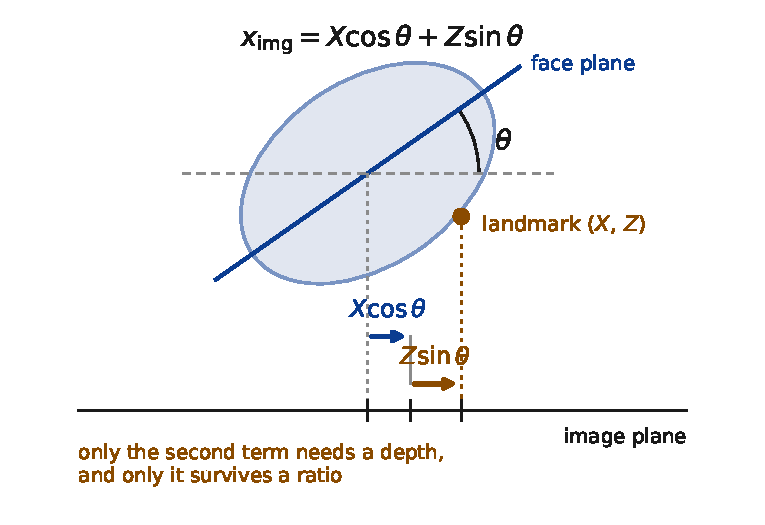
\includegraphics[width=\linewidth]{image/posecorr_a_geometry}
    \caption{}
    \label{fig:posecorr-geom}
  \end{subfigure}
  \hfill
  \begin{subfigure}[b]{0.46\linewidth}
    \centering
    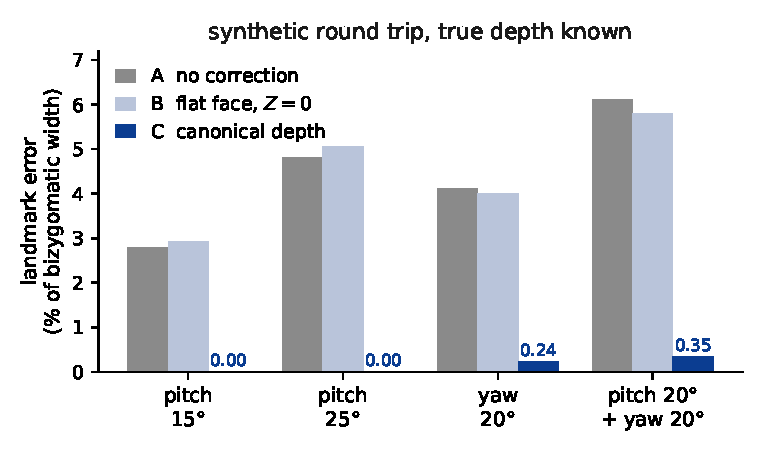
\includegraphics[width=\linewidth]{image/posecorr_b_roundtrip}
    \caption{}
    \label{fig:posecorr-roundtrip}
  \end{subfigure}

  \caption{\textbf{Why the depth term is the whole problem.}
  (\protect\subref{fig:posecorr-geom}) Orthographic geometry of a rotated face.
  The image abscissa decomposes into $X\cos\theta$, an anisotropic scaling of the
  face plane that cancels in a ratio, and $Z\sin\theta$, which does not and which
  is the only term requiring a depth.
  (\protect\subref{fig:posecorr-roundtrip}) Synthetic round trip with the true
  depth known exactly, giving the residual landmark error as a percentage of
  bizygomatic width for the uncorrected, flat-face and canonical-depth arms at
  four head poses. The flat-face arm does not improve on leaving the pose
  uncorrected.}
  \label{fig:posecorr-arms}
\end{figure}

\begin{figure}[t]
  \centering
  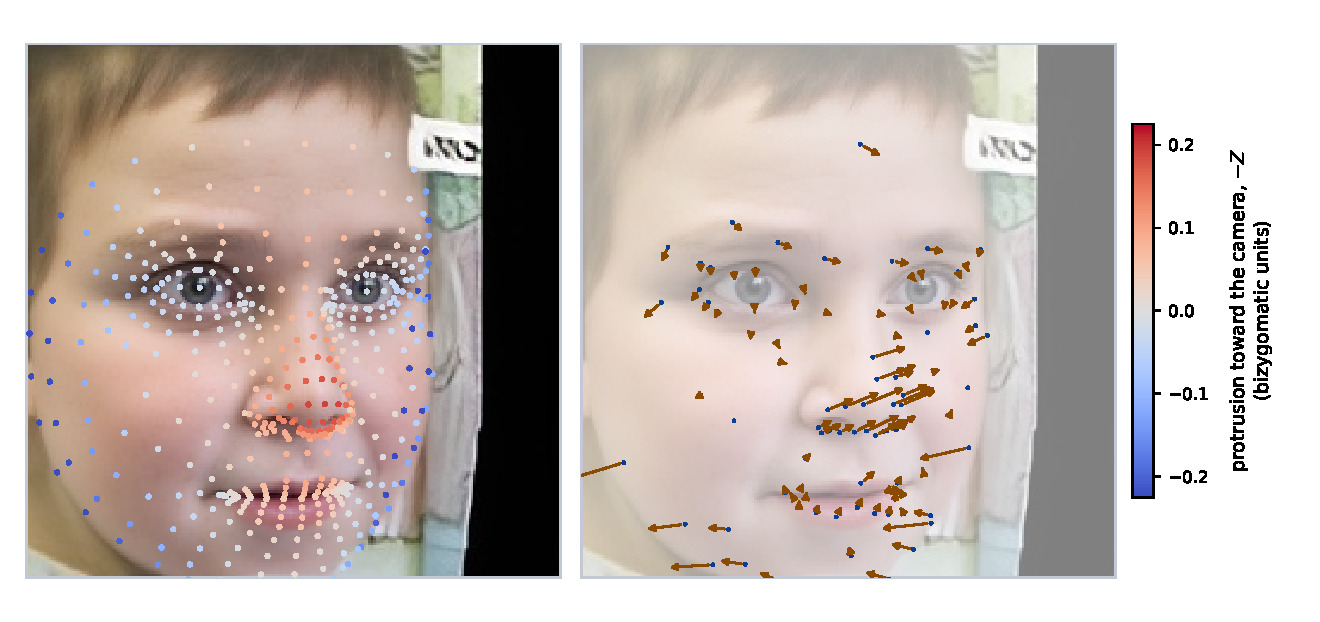
\includegraphics[width=0.92\linewidth]{image/F_posecorr_mechanism}
  \caption{\textbf{What the canonical-depth correction moves on a real
  photograph.} A patient of the Noonan syndrome cohort photographed at
  $18^{\circ}$ of yaw. Left: the depth assigned to each landmark, one constant
  per landmark from the canonical table and identical for every image; the
  per-image depth returned by the detector is not read. Right: the displacement
  the correction applies, drawn at twice its true length, with a median of 2.1\%
  of bizygomatic width and a 95th percentile of 7.0\%. The displacement is the
  $Z\sin\theta$ term and is therefore near zero wherever the face is flat and
  largest across the nose and the malar region. It acts on the measurements that
  depend on depth and leaves the face-plane ratios alone: on this photograph the
  inter-pupillary distance over bizygomatic width changes by $-0.17\%$.}
  \label{fig:posecorr-mech}
\end{figure}

\FloatBarrier

\subsection{Synthetic images reproduce cohort-level geometric phenotypes}

We next asked whether the synthetic faces produced by the trained generators
carry the same geometric phenotype signal as the real photographs they were
trained to imitate. For ten of the rare-disease cohorts we compared 1,727
synthetic images against the 1,647 real images of the same syndromes, passing
both sets through the identical FaceKit pipeline and comparing them on the same
120 measurements. For each syndrome the comparison was restricted to the
measurements its HPO annotations map to, giving 265 syndrome--measurement pairs
in total.

Within each syndrome, the synthetic and real distributions of a measurement were
close. The median absolute Cohen's $d$ between the two sets ranged from 0.048
(Williams--Beuren syndrome) to 0.149 (Noonan syndrome), with an overall
median of 0.075; 84.5\% of all pairs fell below $|d| = 0.2$ and 99.6\% below
$|d| = 0.5$ (Fig.~\ref{fig:syn}\subref{fig:syn-within}). A generator therefore reproduces not only the appearance of a
cohort but the location and spread of the individual measurements taken from it.

A more demanding test is whether the synthetic images preserve what
distinguishes one syndrome from the others, rather than only reproducing each
cohort in isolation. For every syndrome we computed the effect of the focal
cohort against the nine remaining cohorts pooled, separately in the synthetic
and in the real images, and compared the two sets of effects. The direction of
the effect agreed between synthetic and real for a median of 85.6\% of a
syndrome's measurements, and the effect sizes themselves tracked closely
(median Spearman $\rho = 0.912$, median Pearson $r = 0.921$;
Fig.~\ref{fig:syn}\subref{fig:syn-scatter}). Agreement was
weakest for KBG syndrome, Cornelia de Lange syndrome and Noonan syndrome, which
tied at 80.0\% of their 35, 25 and 20 measurements, and complete for Angelman
syndrome, although the latter is mapped to only three measurements.

Across all 265 pairs, 38 (14.3\%) disagreed in sign
(Fig.~\ref{fig:syn}\subref{fig:syn-scatter}, highlighted). These disagreements were
concentrated in the eye region (23 of 126 pairs, 18.3\%) and the eyebrow region
(5 of 30, 16.7\%), and were absent from the philtrum. They were
also almost entirely confined to measurements that barely separate the cohorts
in the real images to begin with: the median $|d|$ measured in real images was
0.047 for the disagreeing pairs against 0.246 for the agreeing ones, and 92\% of
the disagreements occurred where the real effect was below $|d| = 0.2$. Where a
measurement carries no discriminative signal in the real cohort, its sign is not
determined, so these cases indicate an absence of signal to reproduce rather
than a signal reproduced incorrectly. The eyebrow region is the exception worth
naming: KBG syndrome, the weakest cohort overall, disagrees most on inter-eyebrow
distance ($d = +0.228$ synthetic against $d = -0.113$ real), the same measurement
that failed for synophrys above, and for the same reason --- the phenotype lives
in hair rather than in shape, and neither the landmark mesh nor a generator
trained through it represents it.

The one systematic difference between synthetic and real images is dispersion.
The variance of a measurement in the synthetic set was consistently smaller than
in the real set, with a median ratio of 0.87 across all pairs and regional
medians from 0.77 in the chin and jaw and 0.78 in the eyebrow region to 0.95 in
the philtrum (Fig.~\ref{fig:syn}\subref{fig:syn-var}). Synthetic cohorts are therefore narrower than the cohorts they were
trained on: the generators recover where a syndrome sits in measurement space
and how it differs from other syndromes, but under-represent the variation
within it. This should be taken into account when synthetic images are used to
augment training data, since a model trained on them will see a narrower range
of facial morphology than the real population presents.

% Panels generated by manuscript/make_synthetic_panels.py from the post-audit
% facekit_analysis outputs (analysis/failure_modes/ and analysis/per_disease/).
\begin{figure}[t]
  \centering
  \begin{subfigure}[b]{0.5\linewidth}
    \centering
    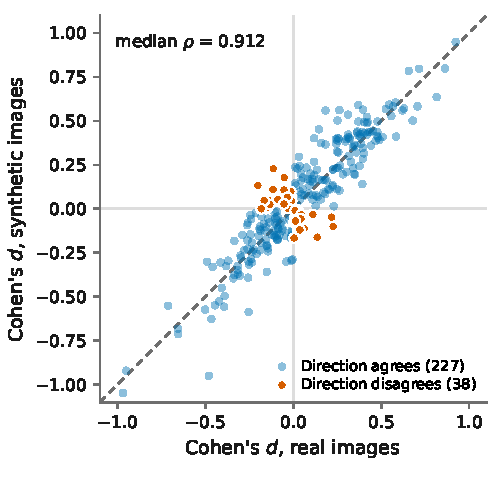
\includegraphics[width=\linewidth]{image/syn_a_effect_scatter}
    \caption{}
    \label{fig:syn-scatter}
  \end{subfigure}
  \hfill
  \begin{subfigure}[b]{0.47\linewidth}
    \centering
    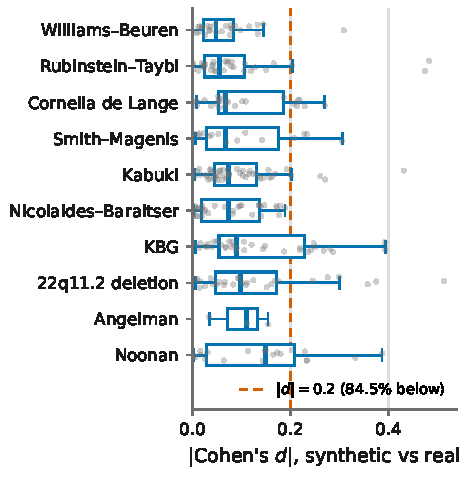
\includegraphics[width=\linewidth]{image/syn_b_within_d}
    \caption{}
    \label{fig:syn-within}
  \end{subfigure}

  \vspace{1em}

  \begin{subfigure}[b]{\linewidth}
    \centering
    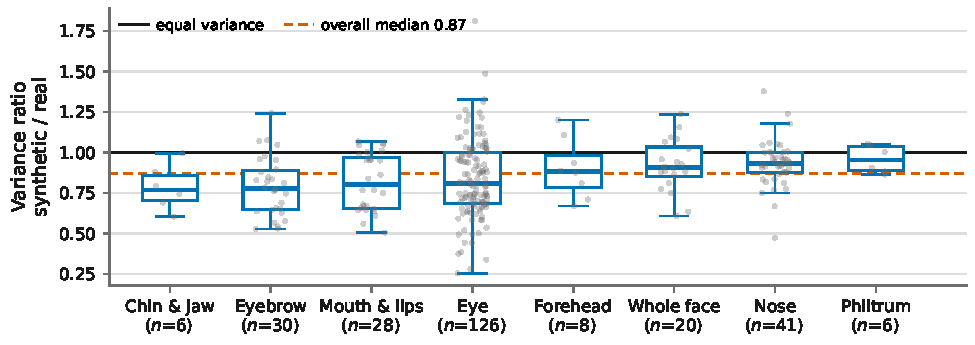
\includegraphics[width=\linewidth]{image/syn_c_variance_ratio}
    \caption{}
    \label{fig:syn-var}
  \end{subfigure}

  \caption{\textbf{Synthetic cohorts reproduce the geometric phenotype of the
  cohorts they were trained on.} All panels cover the 265 syndrome--measurement
  pairs obtained by restricting each of the ten syndromes to the measurements its
  HPO annotations map to. (\protect\subref{fig:syn-scatter}) Effect of the focal
  cohort against the nine remaining cohorts pooled, measured in the synthetic
  images against the same effect measured in the real images; the dashed line is
  equality. Pairs whose effect disagrees in sign between the two are highlighted,
  and lie almost entirely near the origin, where the real effect is itself close
  to zero. (\protect\subref{fig:syn-within}) Within each syndrome, the absolute
  Cohen's $d$ between the synthetic and the real distribution of a measurement.
  Boxes give the median and interquartile range, whiskers extend to
  $1.5\times$ the interquartile range, and individual pairs are drawn behind
  them. (\protect\subref{fig:syn-var}) Ratio of the variance of a measurement in
  the synthetic images to its variance in the real images, by facial region and
  ordered by median. Values below one indicate a synthetic cohort narrower than
  the real cohort.}
  \label{fig:syn}
\end{figure}

\FloatBarrier

\begin{table}[!htbp]
  \centering
  \caption{\textbf{Synthetic images flagged against a real-image reference
  rate.} Each row fixes an operating point by taking the threshold from the
  $p$-th percentile of the distances between held-out real images and the
  training partition, so that $p$ is the false acceptance rate the threshold
  produces among real images of the same cohort; entries give the percentage of
  the 999 synthetic images falling below that threshold. Thresholds are cosine
  distances for the three recognition models and LPIPS distances for the
  perceptual metric. Values at or below $p$ indicate no excess over the
  reference.}
  \label{tab:privacy-far}
  \begin{tabular}{cccccccc}
    \toprule
    & \multicolumn{3}{c}{Identity (\% flagged)} & \multicolumn{3}{c}{Threshold} & Appearance \\
    \cmidrule(lr){2-4} \cmidrule(lr){5-7} \cmidrule(lr){8-8}
    $p$ (\%) & ArcFace & AdaFace & LVFace & ArcFace & AdaFace & LVFace & LPIPS (\% flagged) \\
    \midrule
     1 &  0.10 &  0.10 & 0.00 & 0.3758 & 0.3708 & 0.5146 &  3.8 \\
     2 &  0.50 &  0.20 & 0.00 & 0.4115 & 0.3879 & 0.5450 &  7.7 \\
     5 &  1.30 &  0.70 & 1.50 & 0.4386 & 0.4411 & 0.5946 & 14.1 \\
    10 &  5.01 &  4.00 & 2.60 & 0.4750 & 0.5027 & 0.6249 & 23.0 \\
    20 & 15.02 & 11.61 & 6.71 & 0.5274 & 0.5504 & 0.6673 & 36.1 \\
    \bottomrule
  \end{tabular}
\end{table}

\subsection{Synthetic images do not reproduce training identities}

% Source of numbers: results/Privacy Analysis Summary.pptx (2026-07-14) and the
% face_audit package in results/package.zip. The raw result files
% (nnaa_embeddings.json, nnaa_lpips.json, below_threshold_*.json,
% triplet_accuracy_*.json, calibration_*.json) are not in this repository; every
% value below was checked against the deck. Values marked "read off" come from a
% plot axis and should be replaced with the exact figure from the JSON outputs.

Because the generators are distributed with FaceKit, we finally asked whether
the images they produce disclose the identity of the patients whose photographs
trained them. For the ten rare-disease cohorts we compared 999 sampled synthetic
images against the training partition of each cohort, using as a reference the
611 held-out real images that belong to the same cohorts but were excluded from
generator training. Face recognition embeddings separate these cohorts less
cleanly than they separate adults in the benchmarks they were calibrated on:
across 93 same-person and 111,598 different-person pairs, the two ArcFace
distance distributions were largely distinct but retained a tail overlap of
0.0716 (Fig.~\ref{fig:privacy}\subref{fig:privacy-kde-arcface}), so no threshold
separates identities without error. We therefore did not fix a verification
threshold. Each threshold was instead read off the held-out distances
themselves, so that an operating point is defined by the false acceptance rate
it produces among real images of the same cohort, and the synthetic images were
asked only to stay at or below that rate. A held-out image is subject to the
same recognition errors and to the same coincidental resemblance between
children who share a syndrome as a synthetic image is, so what remains above
this reference is the excess attributable to the generator. The comparison
requires the embedding to rank identities correctly rather than to be
calibrated, and it does: each same-person pair contributes two anchor orderings,
and in 182 of these 186 comparisons (97.8\%) the distance of the same-person
pair was smaller than every different-person distance it was compared against.



Against this reference the synthetic images carried no excess identity signal
(Table~\ref{tab:privacy-far},
Fig.~\ref{fig:privacy}\subref{fig:privacy-far}). At an operating point
corresponding to a 1\% false acceptance rate among real images, 0.10\% of
synthetic images fell below the ArcFace threshold, 0.10\% below the AdaFace
threshold and none below the LVFace threshold. The margin persisted as the
operating point was relaxed: at 5\% the three rates were 1.30\%, 0.70\% and
1.50\%, and at 20\% they were 15.02\%, 11.61\% and 6.71\%. No backbone exceeded
its reference rate at any of the five operating points, and the ordering of the
three models was stable throughout. Within the resolution of these three
recognition models, and at every operating point examined, sampling from the
released generators is therefore not more likely to produce a face matching a
training patient than drawing another real photograph of the same syndrome is.

% Panels are the face_audit plots embedded in results/Privacy Analysis
% Summary.pptx, re-exported by manuscript/make_privacy_panels.py. Regenerate as
% vector PDF from the face_audit outputs when the raw result files are
% available. The overlap-band example panel from slide 7 is deliberately not
% used: it shows identifiable patient photographs.
\begin{figure}[h]
  \centering
  \begin{subfigure}[b]{0.48\linewidth}
    \centering
    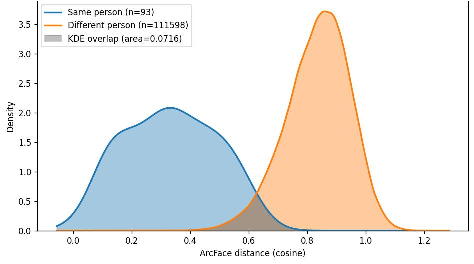
\includegraphics[width=\linewidth]{image/privacy_a_kde_arcface}
    \caption{}
    \label{fig:privacy-kde-arcface}
  \end{subfigure}
  \hfill
  \begin{subfigure}[b]{0.48\linewidth}
    \centering
    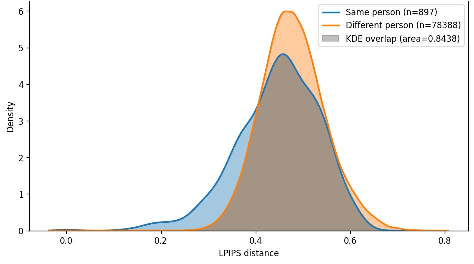
\includegraphics[width=\linewidth]{image/privacy_b_kde_lpips}
    \caption{}
    \label{fig:privacy-kde-lpips}
  \end{subfigure}

  \vspace{1em}

  \begin{subfigure}[b]{0.48\linewidth}
    \centering
    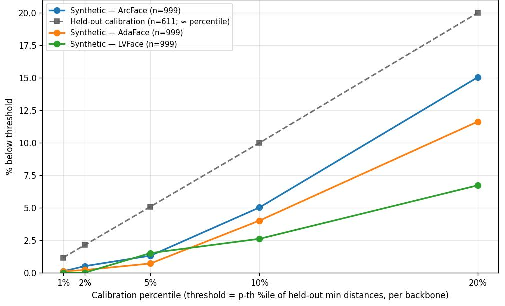
\includegraphics[width=\linewidth]{image/privacy_c_far_identity}
    \caption{}
    \label{fig:privacy-far}
  \end{subfigure}
  \hfill
  \begin{subfigure}[b]{0.44\linewidth}
    \centering
    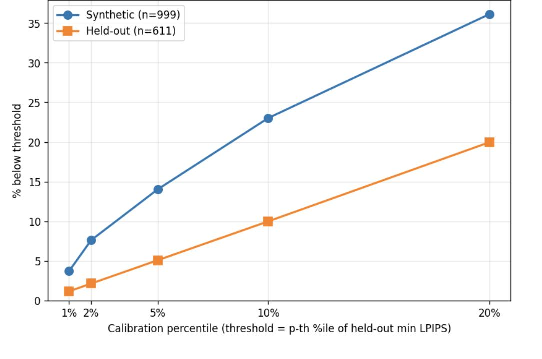
\includegraphics[width=\linewidth]{image/privacy_d_far_lpips}
    \caption{}
    \label{fig:privacy-far-lpips}
  \end{subfigure}

  \caption{\textbf{Privacy assessment of the released generators.}
  (\protect\subref{fig:privacy-kde-arcface}) Distribution of ArcFace cosine
  distances between images of one patient and between images of different
  patients, with the overlap between the two densities shaded.
  (\protect\subref{fig:privacy-kde-lpips}) The same distributions measured with
  LPIPS, which overlap almost completely and therefore carry little identity
  information. (\protect\subref{fig:privacy-far}) Percentage of synthetic images
  falling below a threshold set at the $p$-th percentile of the held-out
  distances, for the three recognition models; the dashed line is the rate the
  same threshold produces among real held-out images.
  (\protect\subref{fig:privacy-far-lpips}) The same comparison measured with
  LPIPS, where the synthetic images are flagged well above the held-out
  reference at every operating point.}
  \label{fig:privacy}
\end{figure}

The picture on the appearance axis is different, and the two must not be
conflated. LPIPS distances between images of one patient and between images of
different patients are almost indistinguishable, overlapping by 0.8438 across
897 same-person and 78,388 different-person pairs
(Fig.~\ref{fig:privacy}\subref{fig:privacy-kde-lpips}); the metric responds to
texture, pose and illumination rather than to identity. Measured with it, the
synthetic images were systematically closer to the training photographs than the
held-out images were, and by a wide margin: 14.1\% of synthetic images fell
below the threshold set at a 5\% reference rate, and 36.1\% below the threshold
set at 20\% (Fig.~\ref{fig:privacy}\subref{fig:privacy-far-lpips}). % read off
A generator trained on a cohort reproduces the acquisition characteristics of
that cohort, and the synthetic images inherit them. Because the same metric
cannot tell two photographs of one patient from photographs of two different
patients, this proximity describes the distribution the images were drawn from
and not the individuals within it.

Both axes are summarized by the nearest neighbour adversarial accuracy.
Computed on embeddings, the privacy loss was $-0.000$ for ArcFace, $-0.002$ for
AdaFace and $-0.006$ for LVFace, with bootstrap confidence intervals that
included zero in all three cases; % read off
synthetic images lie no closer to the training partition than to the held-out
partition. Computed on LPIPS distances the privacy loss was $+0.046$ with a
confidence interval of $[0.031, 0.093]$ that excludes zero, % read off
reproducing in a single number the divergence between the two axes. One feature
of these values deserves comment: the adversarial accuracies themselves ranged
from 0.947 to 0.980 on embeddings, % read off
far above the value of one half that would indicate two indistinguishable sets,
because synthetic faces are globally separable from real ones in recognition
embedding space. The absolute level therefore carries no privacy
interpretation here, and only the difference between the two comparisons does.


\section{Discussion}

FaceKit provides a reproducible and interpretable workflow for transforming facial images into structured geometric phenotype representations. The phenotype-faithfulness analysis showed that most of the mapped measurements deviated from a normative reference in the direction encoded by the corresponding HPO term, although only a subset of these deviations reached statistical significance. At the same time, the results demonstrate that the feature catalogue should be interpreted as a partial geometric representation of facial phenotype rather than a complete translation of HPO descriptions. Individual measurements can be inspected through their landmark definitions and used in cohort-level statistical analyses, but FaceKit is not intended to determine the presence of an HPO term or provide a disease diagnosis.

The privacy assessment supports distributing the pre-trained generators, but with a distinction that should be preserved when the synthetic images are used. On the identity axis, sampling from a released generator was no more likely to produce a face close to a training patient than drawing another real photograph of the same syndrome was, and this held for all three recognition models at every operating point examined. On the appearance axis the synthetic images were clearly closer to the training photographs than held-out real images were. This reflects the acquisition characteristics the generator learned alongside facial morphology rather than the identity of any individual, since the perceptual metric cannot separate two photographs of one patient from photographs of two different patients. The assessment is nevertheless an empirical audit against specific recognition models and a specific perceptual metric, not a formal privacy guarantee: it bounds what these particular measurements can detect, and a stronger attack or a better embedding could in principle detect more.

Several limitations should be considered. First, the reliability of every geometric measurement depends on the accuracy of the underlying facial landmark detector. General-purpose detectors are primarily trained on normative faces and may place landmarks according to learned expectations of typical facial structure when applied to rare-disease faces with substantially different morphology. Errors at this stage propagate directly into all downstream measurements and cannot be corrected through feature design alone. The same limitation applies to any phenotype defined by appearance rather than by shape, as the synophrys result above illustrates: a landmark mesh carries no photometric information and cannot represent hair distribution. Second, some feature failures arise from the choice of geometric formula or normalization scale, as in the full-cheeks result, indicating that normalization strategies may need to be selected separately for different measurements. Third, landmarks estimated from a single two-dimensional image remain sensitive to head pose, facial expression, image resolution, cropping, and acquisition conditions, despite the pose-quality filtering and geometric normalization implemented in FaceKit. These measurements should therefore not be interpreted as equivalent to calibrated three-dimensional facial measurements.

Future development will focus on supporting landmark-detection models adapted to rare-disease faces, refining feature-specific normalization strategies, and incorporating complementary appearance-based representations for phenotypes that cannot be described by geometry alone. Validation in larger cohorts and across demographic and imaging subgroups will also be needed before quantitative ranges can be interpreted clinically.

\bibliographystyle{unsrt}
\bibliography{references}

\end{document}
